
% The API of \sys\ is presented in Section~\ref{ssec:api}. 
\cref{ssec:layout}  discusses \sys's data organization. 
We discuss atomic scans in~\cref{ssec:scans}, and summarize \sys's
normal (maintenance-free) operation flow  in~\cref{ssec:ops}.  
The data structure's maintenance is discussed in~\cref{ssec:rebalance}.
Finally,~\cref{ssec:flush-recovery} discusses data flushes and failure recovery.


\subsection{Data organization}
\label{ssec:layout}

\paragraph{Chunks, funks, and munks.}

\sys's data layout is depicted in Figure~\ref{fig:piwi}.
%Similarly to BTrees and other disk-friendly and cache-friendly data structures~\cite{kiwi}, 
Data resides in chunks, each holding a contiguous key range.
This improves the efficiency of both disk access and memory access, in particular, for  range scans. 
Each chunk's data 
(consisting of keys in the corresponding range and values associated with them) 
is kept on disk (funks, for persistence), and possibly in memory (munks, for fast access). 
Chunk metadata objects are significantly smaller than munks and funks
(typically, less than 1 KB instead of tens of MBs). Hence, at run-time, \sys\ holds them in memory.
In addition, it keeps a volatile \emph{chunk index} -- a sorted map from keys to chunks. 
Index updates are lazy, so it offers only best-effort expedited search.

A chunk %is associated with a funk, % as illustrated in Figure~\ref{fig:funk}. 
consists of two files:  a compacted and sorted  key-value map \emph{SSTable} %(Sorted String Table~\cite{Bigtable2008}) 
and a write \emph{log}. When a funk is created, the \code{SSTable} holds all the chunk's keys with corresponding values, and the \code{log}  is empty.
New key-value pairs are subsequently appended to the unsorted \code{log}. If a key is over-written, it remains in the \code{SSTable} associated with the old value, and is included in the \code{log} with the new one.
That is, the \code{log} is more up-to-date.

\remove{
\begin{figure}[tb]
\centerline{
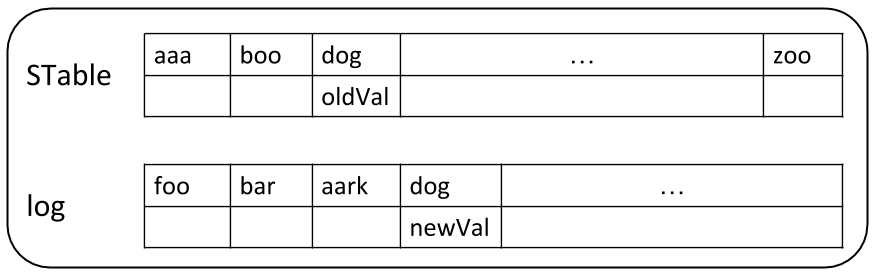
\includegraphics[width=\columnwidth]{funk.png}
}
\caption{A \sys\ funk consists of a sorted \code{SSTable} and an unsorted \code{log} holding the most recent updates.}
\label{fig:funk}
\end{figure}
}

This structure allows us to benefit from sorted searches on the \code{SSTable}, and at the same time
allows for updating chunks without re-writing existing data, thus minimizing write amplification.
As a funk's \code{log}  grows, however, searching becomes inefficient   and  
the funk is no longer compact, i.e., it may contain redundant (over-written) values.
Therefore, once the \code{log}  exceeds a certain threshold, we reorganize the funk
via a process we call \emph{rebalance}, as explained below.
\remove{
In our experiments, we keep the \code{log} \inred{an order of magnitude smaller than \emph{or} 
around the same size as?} the \code{SSTable}  .
}

A subset of the chunks is also cached (as munks) in memory to allow fast access.
Munks are volatile and can be removed and recreated from funks at any time based on an arbitrary replacement policy.
% Thus, multiple \emph{generations} of munks may exist for a chunk throughout its life time.
%Chunks that are not cached are denoted \emph{munk-less}.

%The details of the chunk's metadata structure are deferred to the the supplemental material.

A munk holds key-value pairs in an array-based linked list.  
\remove{
A munk consists of two arrays -- \emph{karray} for keys and \emph{varray} for values. The  \code{karray}  holds a sorted linked list of the chunk's keys
with pointers to values in the \code{varray}. 
}
When a munk is created, some prefix of this array is populated,
sorted by key, so each cell's successor in the linked list is the ensuing cell in the array.
New key-value entries are appended after this prefix.
As new entries are added, they create bypasses in the linked list, and consecutive keys in the
list are no longer necessarily adjacent in the array. Nevertheless, as long as 
a sizable prefix of the  array  is sorted and insertion order is random, bypasses are short in expectation.
\remove{Key removals, in turn, leave obsolete values in the munk, so it is no longer compacted.}
Keys can thus be searched efficiently via binary search on the sorted prefix followed by a short traversal 
of a bypass path at the suffix of the array. This approach was previously used in in-memory data structures,
e.g., Kiwi~\cite{kiwi}.  

As key-value pairs are added, overwritten, and removed, munks and funks need to undergo reorganization. This includes  
(1) \emph{compaction} to garbage-collect removed and overwritten data, 
(2) \emph{sorting} keys to make searches more efficient,  and
(3) \emph{splitting} overflowing chunks.
All reorganizations are performed by \sys's \emph{rebalance} operation.
If the chunk has a munk, then rebalance compacts and sorts the munk, creating a new 
(compacted and sorted) munk instead of the existing one. 
Note that munk rebalance happens in-memory, independently of munk replacement and disk flushes. 
Funks are also compacted and replaced by new funks, albeit less frequently.
Splits  create new chunks as well as new  funks (and possibly munks).

\paragraph{Expediting reads.}
As long as a chunk  is memory-resident, the munk data structure serves both the read-path and the write-path for keys 
in this chunk's range. The chunk metadata is quickly located using the index, and its munk's sorted prefix allows for fast 
binary search. Thus, \sys\ is particularly fast when almost the entire working set is memory-resident. 
We take two measures to mitigate the performance penalty of accessing keys in non-cached chunks.

First, we keep a \emph{row cache} holding popular key-value pairs from munk-less chunks. Note that unlike munks, which cache key ranges, the row
cache holds individual keys, and is thus more effective in dealing with point queries (gets as opposed to scans) with no
spatial locality.
Whereas, popular key ranges %are associated with munks (and 
can be scanned quickly from munks, 
isolated hot keys %are included in the row cache for efficient gets.
can be quickly found using the row cache.

For working sets that are  larger than the available DRAM, these two caches might not suffice, and so a certain portion of reads 
will be served from disk. Here, the slowest step is the sequential search of the \code{log}. 
To reduce \code{log} searches, a chunk with no munk holds a \emph{Bloom filter} for the corresponding funk's \code{log}, 
which eliminates most of the redundant \code{log}  searches.
To reduce the \code{log} search time in case it does happen, 
we further  partition the Bloom filter into a  handful of filters, each summarizing the 
content of part of the \code{log}; this allows us to know not only whether or not to search the 
\code{log}, but also which part of it to search.  
 
\remove{
\paragraph{Chunk metadata structure.}

The metadata structure is given in Algorithm~\ref{alg:chunk}. 
The first field is its \code{status}, which is explained in \cref{ssec:rebalance}  below. 
It next holds a pointer to the appropriate funk, and either a munk or a Bloom filter, as well as a pointer to the next 
chunk in the chunk linked list.
\remove{
It further keeps the generation number of its latest munk, \code{gen}, and a per-generation sequence number,
\code{seq}, which, in case there is an active munk, is the index of the next free cell in the munk's  \code{karray}  and \code{varray}. The chunk's \code{gen} and \code{seq} are stored together in one 64-bit word to allow 
atomic access to both of them. 
}
%It further includes a Bloom filter as explained above.
Finally, the chunk includes locks to synchronize concurrent access by multiple threads, as explained below.

\begin{algorithm}[htb]

\begin{algorithmic}
\State \code{status} \Comment  baby, child, active, asleep, or aged
\State ptr \code{funk} \Comment funk disk address
\State ptr \code{munk} \Comment munk memory pointer
\State ptr \code{next} \Comment next chunk in linked list
%\State int \code{gen} \Comment munk generation
%\State int \code{seq} \Comment sequence number in current generation 
\State ptr \code{bloomFilter} \Comment summary of set of keys in \code{log}
\State asymmetric lock \code{rebalanceLock} \Comment shared/exclusive lock 
\State lock \code{funkChangeLock} \Comment acquired with try\_lock 
% \State \code{$\langle$key, version, done, counter$\rangle$  PPA[threads]} \Comment pending puts
\end{algorithmic}

\caption{Chunk metadata structure.}
\label{alg:chunk}
\end{algorithm}
}

\paragraph{Thread synchronization variables.}

\sys\ supports concurrent execution of all operations.
The replacement of a chunk (due to a split) or rebalance of a funk or munk %(see Section~\ref{ssec:rebalance}) %associated with a given chunk 
must be executed atomically, and moreover, must be synchronized with concurrent puts. 
This is controlled by the chunk's \emph{rebalanceLock}, which is held for short time periods
during chunk, funk, and munk replacements.  It is a shared/exclusive lock, acquired in shared mode by puts and in exclusive mode by rebalance. 
Gets and scans do not acquire the lock. Note that it is safe for them to read from a chunk while it is being replaced. 
Rebalance makes the new chunk accessible only after it is populated. 
Because a chunk is immutable during rebalance (while rebalance lock is in exclusive mode), 
reading either the old or the new version is acceptable.

To minimize I/O, we allow at most one thread to rebalance a funk at a given time; this is controlled by 
the  \code{funkChangeLock}. 
This lock is held throughout the creation of the new funk. 
It is acquired using a try\_lock call, and threads that fail to acquire it do not retry, but instead wait for the winning thread to complete the funk's creation.
%Finally, the chunk holds a data structure called PPA for synchronizing  puts with concurrent scans, as explained in the next section. 

In addition to the chunk list and chunk index, \sys\ keeps a \emph{global version (GV)} for supporting atomic scans (described in the next section) and tracks active threads' activities in the 
\emph{Pending Operations (PO)} array, which has one entry per active thread. 
The PO is used to synchronize puts with scans, as well as for  garbage collection purposes (old 
versions not needed by any active scan can be reclaimed).
We note that using a single pending array to synchronize all operations can cause contention, which we
eliminate in our implementation by tracking the pending puts in per-chunk arrays with per-thread entries as done in~\cite{kiwi}.
%(see the supplemental material for details).%~\cref{sec:impl}). 

\subsection{Multi-versioning for atomic scans}
\label{ssec:scans}

% \paragraph{Multi-versioning.}

We support atomic scans via multi-versioning using the system-wide global version, GV. 
A scan operation creates a \emph{snapshot} associated with GV's current value by incrementing GV, 
which signals to ensuing put operations that they must not overwrite values  with the highest
version smaller than the new GV value.
This resembles a \emph{copy-on-write} approach, which virtually creates a snapshot by 
indicating that data pertaining to the snapshot should not be modified in place.  

To allow garbage collection of old versions, \sys\  tracks snapshot times of 
active scans in the pending operations array, PO.
The compaction process that runs as part of rebalance removes old versions that are no longer required for any  
scan listed in PO. Specifically, for each key, it removes all but the last version that is smaller than the minimal
scan entry in PO and also smaller than the value of GV when the rebalance begins. 

\remove{
For linearizing (i.e., determining an order on) updates, we associate each key-value pair written to the data store 
with a unique-per-key timestamp.
This timestamp is composed as a tuple $\langle$ver, gen, seq$\rangle$, where \emph{ver} is  the version read from GV 
(recall that GV is only incremented upon scans and hence might remain unchanged across multiple puts),
\emph{gen} is the generation of the target chunk's last created munk  (which may or may not still exist), 
and seq is the running sequence number of values inserted to the chunk in the current generation.
}

% \paragraph{Concurrent puts and scans.}

A put obtains a version number from GV without incrementing it. Thus, multiple puts may write values with the same version, each over-writing the previous one. 
%Ordering concurrent puts with the same key and version is discussed in the next section where we elaborate on the put operation's logic.

%A scan begins by fetching-and-incrementing GV.
If a put obtains its version before a scan increments GV, then the new value must be included in the scan's snapshot. 
However, because the put's access to the GV and the insertion of the new value to the chunk do not occur atomically,
a subtle race may arise. Consider a put operation that obtains version $7$ from GV and then stalls before
inserting the value to the chunk, while a scan obtains version $7$ and increments GV to $8$. The scan then proceeds 
to read the appropriate chunk and does not find the new value although it should be included in its snapshot.

To remedy this, we have puts announce (in PO) the key they intend to change when beginning their operations, and have scans wait for relevant pending puts to complete as explained below.
This mechanism is a simplification of the non-blocking put-scan synchronization employed (and proven correct) in~\cite{kiwi}.

%For symmetry, get operations synchronize with puts the same way that scans do. 

\remove{
A put operation takes hold of the chunk's \code{rebalanceLock} in shared mode, 
then publishes itself in the PO, gets a version by reading GV, updates its version in PO,  
and releases the chunk lock. 
}


\remove{
% Simplified PPA
  The per-chunk PPA is used to synchronize pending puts  with ongoing scans. It holds an entry for every active inserting thread, consisting of a \code{key},  a \code{version}, 
 a \code{done} bit indicating whether the update has been completed, and a monotonically increasing 
 \code{counter} to avoid ABA scenarios.
 
A put operation first registers itself in the appropriate chunk's PPA entry with the key it intends to put.
It then reads GV and sets the version field in its PPA entry to the read version. 
After completing the actual put (in the appropriate munk and/or funk), it sets the \code{done} bit.
A scan, in turn, scans the PPA in addition to the chunk's data 
(\code{karray},  \code{log} or \code{SSTable}  ). If it finds a pending put
of a relevant key that is not yet associated with a version, it waits for the version to be assigned. 
Once the version is assigned, if it is the highest version for this key that does not exceed its scan time, 
it waits for the \code{done} bit to be true or for the the \code{version} to change again, at  which point
it reads the value from the appropriate munk or funk.
}


\subsection{Normal operation flow}
\label{ssec:ops}

\paragraph{Get and put.}

Algorithm~\ref{alg:ops}  presents pseudocode for the normal operation flow, without rebalance.
Both get and put begin by locating the target chunk using the \code{lookup} function. In principle, this can be done by traversing the chunk list, but that would result in linear search time. To expedite the search,   \code{lookup} searches the index first. However, index updates are lazy -- they occur after the new chunk is already
in the linked list -- and therefore the index may return a stale chunk that has already been replaced by rebalance or miss newly added chunks. To this end, the index search is repeated with a smaller key in case the index returns a stale chunk, and the index search is supplemented by a linked-list traversal. A similar approach was used in earlier works~\cite{kiwi,tdls}. 

% \code{get}'s optional \code{ver} parameters is used by scans to indicate the snapshot time; when not provided \code{get} simply returns the latest version it finds. A scan is executed by 

\remove{
The operations then proceed to synchronize via the \code{PO} 
as described in Section~\ref{ssec:scans} above. Namely, \code{put}  publishes itself 
in the \code{PO}.
 , and  \code{get} 
checks the \code{PO}  for new potentially relevant puts and waits for them to complete. 
} 

% A \code{scan} operation creates a snapshot, which then allows iterating 

\begin{algorithm}[tb]
\begin{algorithmic}[1]{}
\Procedure{get}{key}	
		\State $C \leftarrow$ \code{lookup(key)}

%		\State $T \leftarrow  \{ \langle \code{th}, i \rangle : \code{C.PPA[th].key = key }  $ 
%		\Statex \hspace{21mm}	$ \wedge \; \code{C.PPA[th].counter} = i \}$ 



%		\code{th} $\in T$,  
%		\Statex  \hspace{21mm}		$C.$\code{PPA[th].done} $\vee$ \code{$C$.PPA[th].ver $>$ gv}
		\If{$C$.\code{munk}} 
			\State search \code{key} in $C$.\code{munk} linked list;  return 
		\EndIf
		\State search \code{key} in row cache; return  if found
		\If{\code{key}$\in C.$\code{bloomFilter}}  
			\State	search \code{key} in \code{funk.log}; return  if found
		\EndIf
		\State	search \code{key} in \code{funk.SSTable}; return  if found
		\State return NULL	
\EndProcedure
\Statex
\Procedure{put}{key, val}	
		\State $C \leftarrow$ \code{lookup(key)}
		\State lockShared($C$.\code{rebalanceLock})
		\State  \code{PO[i]}  $\leftarrow$ \code{$\langle$put, key, $\bot \rangle$ }
			 \Comment publish  thread's presence 
		\State \code{gv} $\leftarrow$ \code{GV}   \Comment fetch and increment global version
		\State  \code{PO[i]}  $\leftarrow$ \code{$\langle$put, key, gv$\rangle$ }
			\Comment and write in \code{PO}
%		\Statex \Comment atomically allocate entry in munk and get its pointer
%		\State \code{$\langle$gen, seq$\rangle$ } $\leftarrow$ F\&I ($C$.\code{$\langle$gen, seq$\rangle$})
%		\State \code{munk} $\leftarrow$ $C$.\code{munk} \Comment read atomically with \code{gen}
		\Statex \Comment write  to funk log, munk (if exists), and row cache  
		\State append \code{$\langle$key, val, gv$\rangle$} to \code{funk.log}
		\If{$C$.\code{munk}} 
			\State add  \code{$\langle$key, val, gv$\rangle$} to $C$.\code{munk}'s linked list
%			\State \code{munk.karray[seq]}  $\leftarrow$ \code{key}
%			\State \code{munk.varray[seq]}  $\leftarrow$ \code{val}
%			\State link \code{munk.karray[seq]} into   \code{munk.karray}
		\Else
		\State update \code{$\langle$key, val$\rangle$} in row cache (if key is present)
		\EndIf
		\State unlock($C$.\code{rebalanceLock})
		\State \code{PO[i]}  $\leftarrow \bot$ 
\EndProcedure
\Statex
\Procedure{scan}{key1, key2}
		\State  \code{PO[i]}  $\leftarrow$ \code{$\langle$scan, key1, key2, $\bot \rangle$ } \Comment publish scan's intent 
		\State \code{gv} $\leftarrow$ \code{F\&I(GV)}   \Comment read global version
		\State  \code{PO[i]}  $\leftarrow$ \code{$\langle$scan, key1, key2, gv$\rangle$ }
		\Comment publish version in PO
		\State  $T \leftarrow $  PO entries updating keys in range [\code{key1, key2}] 
		\State wait until $\forall t \in T, t$  completes or has a version $>$   \code{gv}
		\State $C \leftarrow$ \code{lookup(key1)}
		\Repeat
%			\If{$C$.\code{munk}} 
				\State collect from $C$.\code{munk} or $C$.\code{funk} (\code{log} and \code{SSTable})
				\Statex \hspace{1cm} max version $\le$\code{gv} for all keys in [\code{key1, key2}] 

%			\Else
%				\State get max version $\le$\code{gv} for keys in $C$.\code{funk}
%			\EndIf
			\State $C \leftarrow C$.\code{next} 
		\Until{reached \code{key2}}
%		\State return collected values
\EndProcedure	
\end{algorithmic}
\caption{\sys\ normal operation flow for thread \code{i}.}
\label{alg:ops}
\end{algorithm}


%Once all relevant \code{put}s that were pending when a \code{get}  began complete, the 
A \code{get} proceeds without synchronization. If the chunk has a munk,  \code{get}   locates the key in it by first using binary search in its sorted prefix, and then traversing linked list edges. 
Otherwise, the \code{get} searches the key in the \code{row cache}. If it is not found, it queries 
the \code{Bloom filter} to learn whether the key might be present in the target chunk's  
 \code{log}, and if so, searches for it there.  Finally, if the key is not in any of these places, it searches
 the  \code{SSTable}.

\remove{
A \code{put} proceeds by allocating the next free entry in 
the munk to its value by atomically fetching-and-incrementing the chunk's 
$\langle$ \code{gen}, \code{seq} $\rangle$ pair. It obtains the \code{munk} atomically with 
the read of \code{gen} in order to ensure that \code{seq} indexes the correct array. 
This can be done by re-reading  \code{gen} or by loading one object that references both.
} 

Upon locating the chunk,  a \code{put} grabs its \code{rebalanceLock} in shared mode to ensure that the chunk is not being rebalanced during the \code{put} operation. It then registers itself in PO with the key it intends to put,
reads GV and sets the version field in its PO entry to the read version. 
The \code{put} then proceeds to write the new key-value pair to the  funk's \code{log} and to the 
munk (if one exists). 
If the funk has no munk and the row cache contains an old value of the key, the row cache is then updated.
The munk and funk are multi-versioned to support atomic scans, 
whereas the row cache is not used by scans and holds only the latest version of each key. 
In case the put's version is the same as the current latest one, it over-writes the current one in the munk
but appends a new one in the funk's log. 

\remove{
We note that in case multiple puts update the same key concurrently, a race may arise: 
two concurrent puts may update the funk and munk (or the funk and row cache) in  different orders,
and so the latest update to one will not coincide with the latest update to the other. 
This can be addressed, for example, by locking
keys. 
}
A per-chunk monotonically increasing counter is used to determine 
the order of concurrent put operations updating the same key (similarly to~\cite{kiwi}).
We  enforce updates to occur in order of version-counter pairs by attaching it to the value in the munk, 
\code{PO}, the funk, and the row cache.
Following a split, the new chunks inherit the counter from the one they replace.  
Finally, a put unregisters itself from \code{PO}, indicating completion, 
and releases the chunk's lock .

\paragraph{Scan.}
A scan first publishes its intent to obtain a version in \code{PO}, to 
signal to concurrent rebalances to not remove the versions it needs. It
fetches-and-increments GV to record its snapshot time \code{gv},  
and then publishes its key-range and \code{gv} in \code{PO}.
Next, the scan waits for the completion of all pending puts  
that might affect it  -- these are puts of keys in the scanned key range, which either do not have a version yet or have versions lower than the scan time.
This is done by busy waiting on the PO entry until it changes; monotonically increasing counters are used 
in order to avoid ABA races. 

Then it collects the relevant values from all chunks in the scanned range.
Specifically, if the chunk has a munk, the scan reads from it, for each key in its range, 
the latest version of the value that precedes its snapshot time.
Otherwise, the scan collects all the relevant versions for keys in its range from both 
the \code{SSTable}   and the \code{log} and merges the results.
Finally, the scan unregisters from \code{PO}.
 %are executed by calling \code{createSnapshot(fromKey, toKey)} 
%and then iterating over the key range with \code{next} calls.

\subsection{Rebalance}
\label{ssec:rebalance}

\inred{
Rebalance is used to improve data organization in a funk or munk by removing old versions that are no longer needed 
for scans, removing deleted items, and sorting all the keys in the chunk. It is typically triggered when the munk (funk)
exceeds a capacity threshold.   
%It can be triggered either by a thread attempting to access the chunk or a dedicated background thread.
In case a chunk has a munk, rebalance reorganizes only the munk, since all searches are served by it. 
The respective funk is reorganized much less frequently, merely in order to bound the log's growth. 
Both types of rebalance operations create new munks (funks) rather than reorganize in-place, 
in order to reduce impact on the concurrent accesses. At the end of data reshuffle, \sys\/ flips the 
chunk's reference to the new munk or funk.

\sys\/ executes munk rebalance in the context of the application thread that triggered it. The algorithm blocks 
the puts to the munk throughout the rebalance, so that the concurrent gets and scans can exploit the munk's 
immutability and proceed without synchronization. This is done through the chunk's \code{rebalanceLock} -- 
a shared/exclusive lock that is acquired in shared mode by puts, and in exclusive mode by rebalance. 

The algorithm iterates through the \code{PO} to collect the minimum version number among the active scans that cannot be reclaimed yet. 
Since each rebalance operates on a single chunk with a known key range, scans targeting non-overlapping ranges are ignored.
If a scan published its intent in the \code{PO}  but published no version yet, the rebalance waits until the version is published. 
When the new munk is ready, the procedure flips the munk reference
and releases \code{rebalanceLock}.

Funk rebalance creates an (SSTable, log) pair. \sys\/ executes this procedure in a dedicated daemon thread. If the chunk has a munk, 
the most efficient way of performing funk rebalance is by creating the new SSTable using the munk's content (after filtering obsolete versions) and then truncating the log.
%the most efficient way of performing funk rebalance is through munk rebalance that is followed by the log's truncation and the
%reordered munk's flush to the new SSTable. 
Otherwise, the new SSTable is created by merging the old SSTable with its log. 
This procedure involves I/O and may take a long time, so we do not block puts for the most of its duration. The puts that happened 
after the merge started get logged but do not contribute to the merge result. At the end, \sys\/ performs a catch-up: 
(1) new puts are blocked using the \code{rebalanceLock},
(2) the unaccounted puts are copied to the new log, 
(3) the funk reference is flipped, and (4) \code{rebalanceLock} is released. 
Simultaneous rebalance of the same funk by two threads is prevented in order to avoid redundant work,
through a separate exclusive lock. %s\code{funkChangeLock}, 

\remove{
\paragraph{Splits and chunk life cycle.}

As noted above, as a result of a rebalance operation, a chunk may undergo three types of changes: munk rebalance, funk rebalance, and split. 
The latter affects the chunk object as well as the munk (if exists) and the funk.

In case of a munk rebalance, the chunk is immutable throughout the rebalance operation.
%, and put operations targeting that chunk must wait or help rebalance to complete. 
In this simple case, the chunk's status changes to \emph{asleep} (indicating that it is immutable)
when rebalance begins, and changes back to \emph{active} when rebalance ends. 
Note that the asleep status is tantamount to the \code{rebalanceLock} being held in exclusive mode.

Since funk rebalance involves I/O, it may take a long time, and so we refrain from blocking puts for its entire 
duration. In this case, the chunk becomes asleep after most of the funk is populated, and 
changes back to active after we migrate the \code{log}'s new tail to the new chunk and swing the funk pointer in the chunk.
}

\paragraph{Splits and chunk life cycle.} 
\begin{figure}[tb]
\centerline{
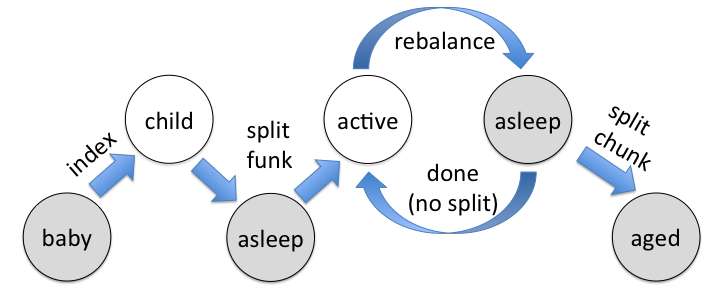
\includegraphics[width=.8\columnwidth]{state-diagram.png}
}
\caption{Chunk life cycle; immutable states are grey and mutable ones are white.
Chunk splits  create new chunks in immutable \emph{baby} status, which changes to the mutable \emph{child} state once they 
are indexed. When the appropriate funks are created, the chunks become \emph{active}. All rebalance operations go through an 
\emph{asleep} state when the chunk is immutable.}
\label{fig:chunklife}
\end{figure}

If a munk rebalance exceeds the data threshold in a new munk, it resorts to chunk split. The algorithm works as 
follows: (1) split the munk into two ordered halves (as an optimization, reuse the first half already
created by the normal rebalance), (2) create two new chunks, each referencing a different new munk
but temporarily sharing the same funk, (3) insert the new chunks into the list after the old chunk, then insert them 
into the index, (4) remove the old chunk from the index and the list, (5) split (in the background) the shared 
funk in two, using the new munks, and update the funk references. Note that the old chunk remains immutable
throughout the process. 

In order to guarantee correctness of this multi-step process, we model a chunk's life cycle as a finite state machine, 
depicted by Figure~\ref{fig:chunklife}. A new chunk is created in \emph{baby} state, in which it is immutable. Once added 
to the index, a chunk transitions to \emph{child} state, in which it is mutable but cannot be rebalanced yet. Finally, when 
a chunk gets its own funk it becomes \emph{active} -- i.e., eligible for all operations. A chunk that has been split into 
two new chunks becomes \emph{aged} -- a state in which it remains immutable but can serve the gets and the scans 
that are concurrently accessing it via the index. Once it gets removed from the chunk list and has no outstanding
reads, it can be disposed. We omit the formal correctness proof for lack of space; see~\cite{kiwi} for similar proofs.   

Underflowing neighbor chunks (e.g., following a massive delete) can be merged following a similar protocol. 
Our current \sys\/ prototype does not implement this feature yet. 
%Merges can be handled the same way by making the two merged munks immutable for the duration of the switch; 
%we do not implement this feature in our prototype.
}

\subsection{Disk flushes and recovery}
\label{ssec:flush-recovery}

All puts write to the funk log, regardless of whether the chunk has a munk. Like most popular KV-stores, \sys\ supports 
two modes of operation -- \emph{synchronous} and \emph{asynchronous}. With the former,  updates are persisted to disk 
before returning to the user, and so a user is ensured when its operation completes that the written data will survive failures. 
The drawback of this approach is that it is roughly an order-of-magnitude slower than the asynchronous mode in existing KV-stores 
like RocksDB~\cite{RocksDB} as well as in \sys. In asynchronous mode, updates to funk logs occur in the OS cache but might 
not be physically persisted until the explicit \code{fsync} call.  Asynchronous I/O reduces write latency and increases throughput, but 
may lead to loss of data that was written shortly before the crash. The tradeoffs between the two approaches are 
well known and the choice is typically left to the user.

\paragraph{Recovery semantics.}
In the synchronous mode, 
%every put operation performs a flush after writing the data in the appropriate funk's \code{log}, and then returns. 
%This ensures that 
the funks always reflect all completed updates. In this case, recovery is straightforward: we simply construct
the chunks linked list and chunk index from the funks on disk, and then the database is immediately ready to serve new requests, populating munks and Bloom filters on-demand.  

In the asynchronous mode, some suffix of the  data written before a crash may be lost, but we  
ensure that the data store consistently reflects a \emph{prefix} of the  values written.
For example, if \code{put(k1, v1)} completes before \code{put(k2, v2)} 
is invoked and then the system crashes, then following the recovery, 
if \code{k2} appears in the data store, then \code{k1} must appear in it as well. 
%conversely, if the update of \code{k1}  is lost, \code{k2}  must be also excluded.
Such recovery to a \emph{consistent snapshot} of the data store is important, since later updates may depend on earlier ones. 

\paragraph{Checkpointing for consistent recovery.}
To support recovery to a consistent snapshot in asynchronous mode, we use a background process to
periodically create and persist \emph{checkpoints} of the data store.
The checkpointing process creates a snapshot similarly to the atomic scan mechanism. That is, 
it begins by fetching-and-incrementing GV to obtain a 
 snapshot version \code{gv}.  Next, 
it synchronizes with pending puts via PO to ensure that all puts with smaller versions are complete. 
It then flushes all the pending writes to disk (using an \code{fsync} call). 
Once the flush is complete, it writes \code{gv} to a dedicated \emph{checkpoint file} on disk,
indicating that all updates pertaining to versions smaller than or equal to this version have been persisted.
Note that some puts with higher versions than \code{gv} might be reflected on disk while others are not. 

Recovery in \sys\ is lazy, keeping all data on disk, and 
allowing it to be fetched from disk into munks  on demand in the course of the normal operation mode. 
To ensure consistency, following a recovery,  
retrievals from funks should ignore newer versions that were not included in the latest completed checkpoint before the crash. 
This must be done by every operation that reads data from a funk, namely \code{get} or \code{scan} from a chunk without a munk, 
funk rebalance, or munk load. 

To facilitate this check, we distinguish between pre-crash versions and new ones created after recovery using \emph{epoch numbers}. 
Specifically, a version is split into an epoch number (in our implementation, the four most-significant bits of the version) and a per-epoch version number. 
Incrementing the GV in the normal mode effectively increases the latter.
The recovery procedure increments the former and resets the latter, so 
versions in the new epoch begin from zero. 

We maintain a \code{recoveryTable} mapping each recovered epoch to its last checkpointed version number. 
For example, Table~\ref{table:recovery} shows a possible state of the recovery table after two recoveries, i.e., during epoch $2$. 

\begin{table}[h]
\begin{center}
\begin{tabular}{ll}
epoch & last checkpointed version \\
\hline
0 & 1375\\
1 &  956\\
\end{tabular}
\end{center}
\caption{Example recovery table during epoch $2$.}
\label{table:recovery}
\end{table} 
 
 \remove{
Every read from a funk  %(during get,  scan, funk rebalance,  or munk load) 
refers to the recovery table in order to identify versions that should be ignored -- 
these are versions from old epochs that exceed the checkpoint number for their epoch. 
}
%\paragraph{Recovery procedure.} 
The recovery procedure is very simple: it reads the checkpoint time from disk, loads the \code{recoveryTable} into memory, adds a new row to it with the last epoch and latest checkpoint time, and persists it again. It then increments the epoch number, and resumes normal operation with version number $0$ in the new epoch.




\remove{
\subsection{\sys\ operations}
\label{ssec:ops}

\inred{Consider if we want full pseudocode}
}








